\documentclass[a4paper]{article}
\usepackage{algorithmicx}
\usepackage{algpseudocode}
\usepackage{graphicx}
\usepackage{vmargin}
\usepackage[utf8]{inputenc}
\usepackage{mdwlist}
\setpapersize{A4}
\setmargins{2.5cm}       % margen izquierdo
{1.5cm}                        % margen superior
{16.5cm}                      % anchura del texto
{23.42cm}                    % altura del texto
{10pt}                           % altura de los encabezados
{1cm}                           % espacio entre el texto y los encabezados
{0pt}                             % altura del pie de página
{2cm}                           % espacio entre el texto y el pie de página

\begin{document}
\section{Caballos salvajes}
\subsection{Problema a resolver}
El problema est\'a dado por encontrar, dado un tablero de $n$ x $n$ posiciones y una cantidad $k$ de caballos (en el contexto del ajedrez) ubicados en dicho tablero, una posición del tablero a la cual puedan llegar todos los caballos con la mínima cantidad de movimientos. Cuando decimos \textit{m\'inima cantidad de movimientos}, nos estamos refiriendo a que, la suma de los movimientos que hace cada caballo para llegar a la posici\'on que devolvemos, tiene que ser menor o igual a la suma denotada por cualquier otra posición del tablero.
\newline Vale aclarar que este problema no siempre tiene solución. No existe una solución cuando no existe \textit{\textbf{ninguna}} posición del tablero a la cual podemos llevar a todos los caballos.
\newline A continuación vamos a ver algunos ejemplos de instancias del problema con sus respectivas soluciones. Para que se entiendan bien las imágenes, aclaramos que el primer tablero de cada una de ellas representa una instancia particular del problema y cada tablero consecutivo representa un movimiento de uno o varios caballos.
\begin{figure}[h!]
\centering
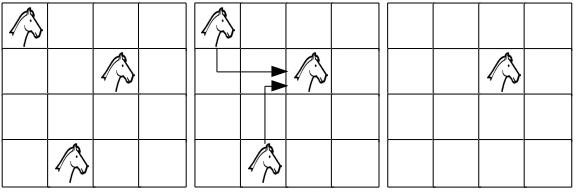
\includegraphics[scale=0.7]{instancia1.jpg}\caption{Problema con $n = 4$, $k = 3$, caballos en (1, 1), (2, 3), (4, 2). Soluci\'on: posición: (2, 3), cantidad de movimientos: 2.}
\vspace{0.2cm}
\centering
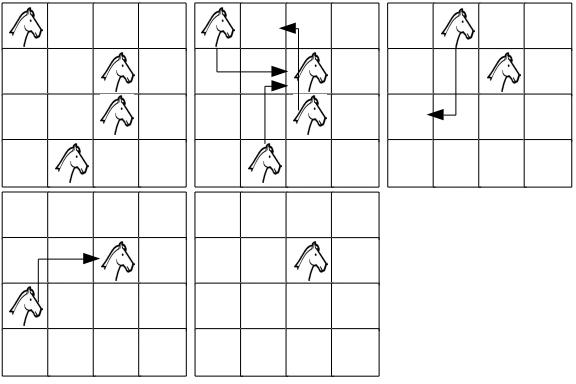
\includegraphics[scale=0.7]{instancia2.jpg}\caption{Problema con $n = 4$, $k = 4$, caballos en (1, 1), (2, 3), (4, 2), (3, 3). Solución: posición (2, 3), cantidad de movimientos: 5.}
\end{figure}

\begin{figure}
\centering
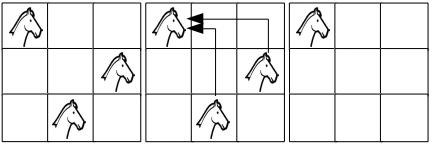
\includegraphics[scale=0.7]{instancia3.jpg}\caption{Problema con $n = 3$, $k = 3$, caballos en (1, 1), (2, 3), (3, 2). Solución: posición (1, 1), cantidad de movimientos: 2.}
\end{figure}

\begin{figure}
\centering
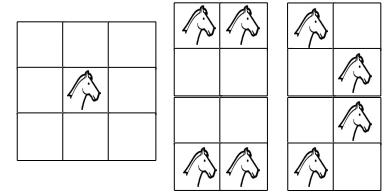
\includegraphics[scale=0.7]{instsinsol.jpg}\caption{El objetivo de esta imagen es analizar las instancias del problema para las cuales no existe solución. El primer tablero de $n = 3$ podemos observar que tiene un caballo (o más) en la posición (3, 3). Si agregáramos un caballo en \textit{otra} posición del tablero, ya no existiría solución al problema. Esto sucede porque un caballo en la posición (2, 2), en un tablero de $n = 3$, no puede moverse hacia ninguna otra posición debido a la particularidad de su movimiento, el cual lo obliga a moverse siempre dos posiciones en la misma dirección. Algo similar pasa con los tableros de $n = 2$, donde tampoco se pueden mover los caballos por falta de posiciones en el tablero. Por lo tanto, los cuatro tableros de la derecha representan instancias del problema para las cuales no existe solución.}
\end{figure}

\subsection{Resolución}
Para resolver el problema, vamos a saber de antemano (más adelante explicaremos cómo), cuál es la cantidad mínima de movimientos que debe hacer cada caballo para llegar a una posición partiendo desde su posición inicial (vamos a llamar a esta cantidad $c_{r}^{p}$ para un caballo $r$ y una posición $p$). Sabiendo esto, la dificultad de querer dar una solución (si es que existe) claramente disminuye bastante. La solución, si es que existe, estaría dada por una posicion $t$ del tablero, tal que la suma $S_t = c_{1}^{t} + c_{2}^{t} + ... \ + c_{k}^{t}$ es menor o igual que $S_t'$ para toda posición $t'$ en el tablero. Es decir, la posición del tablero que minimiza la suma de los movimientos requeridos para llegar a ella partiendo de las posiciones iniciales de cada caballo, junto con la cantidad de movimientos (podemos pensar a la solución como una tupla). Basícamente el problema pasaría a ser sacar el mínimo de $n^2$ sumas, lo cual no parece complicado.
\newline La idea es tener los $c_{r}^{p}$ en una matriz $M$ de $k \ $x $ n \ $x $ n$, de manera tal que, si $p = (i, j)$ una posición en el tablero y $r$ un caballo, entonces $M[r][i][j] = c_{r}^{p}$. Entonces después de llenar esa matriz, vamos a tomar para cada posición $(i, j)$ del tablero, la suma sobre todos los caballos (es decir $M[1][i][j] + M[2][i][j] + ... + M[k][i][j]$) y luego tomar el mínimo de todas esas sumas junto con la posición que denota dicho mínimo, como bien dijimos antes.
\newline
\newline Veamos ahora, una idea a grandes rasgos sobre como llenar M para algun caballo $r$, luego daremos el pseudocódigo para que quede mas claro.
\newline Inicialmente $r$ está en una posición $(i_0, j_0)$, por lo tanto $M[r][i_0][j_0]$ tiene que valer 0 ya que no es necesario hacer ningún movimiento por parte de $r$ para llegar a $(i_0, j_0)$ porque es ahí donde empieza estando. Lo que hacemos ahora es fijarnos, a qué posiciones del tablero puede ir $p$ desde $(i_0, j_0)$ con un solo movimiento. Estas posiciones van a ser a lo sumo 8 (ver imagen abajo), las guardamos en una lista y ahora repetimos el mismo procedimiento, solo que pensamos a $r$ como si hubiera empezado en cada una de esas 8 posiciones. A la hora de llenar la matriz en cada repetición del proceso, ya no vamos a poner ceros como hicimos con $M[r][i_0][j_0]$, si no que vamos a ir incrementando (al final de cada iteración) un valor $v$ que será el asignado a la matriz. Dejaremos de iterar cuando, para toda posición $(i, j)$ del tablero, hayamos asignado a $M[r][i][j]$.

\begin{figure}[h!]
\centering
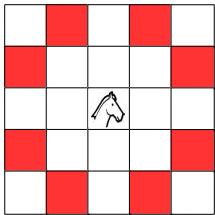
\includegraphics[scale=0.5]{las8.jpg}\caption{El caballo está en $(3, 3)$ y puede ir a las posiciones $(1, 2), (1, 4), (2, 1), (2, 5), (4, 1), (5, 2), (4, 5), (5, 4)$}
\end{figure}

\vspace{0.3cm}
\noindent Hay algunos detalles importantes a tener en cuenta sobre lo explicado arriba. El principal problema es el de los casos repetidos ya que, puede suceder (y de hecho sucede), que al procesar las posiciones a las cuales puedo saltar partiendo desde otra posición, obtenga una posición $p_m$ que ya marqué en la matriz (ver imagen abajo). En este caso decidimos no procesar a $p_m$ y seguir con las otras.

\begin{figure}[h!]
\centering
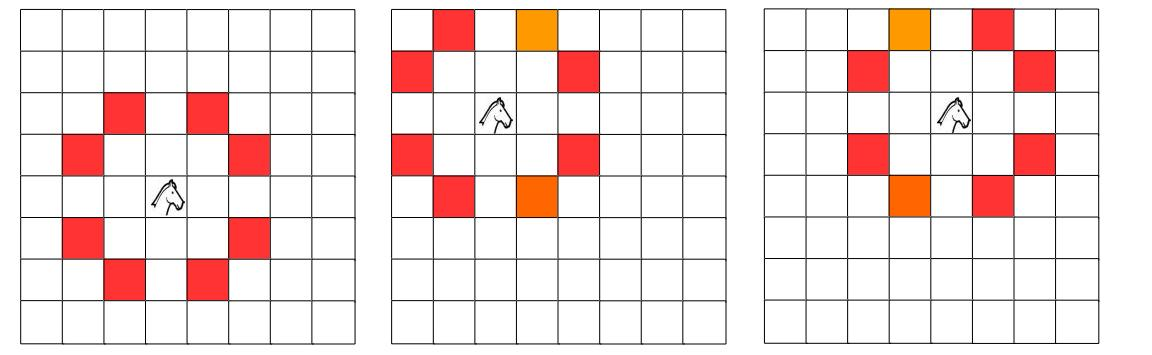
\includegraphics[scale=0.4]{las8repetidas.jpg}\caption{En el primer tablero el caballo está en su posición inicial y mostramos las posiciones posibles a las cuales puede saltar. En el segundo y tercer tablero el caballo ya saltó a una posición y, nuevamente mostramos las posiciónes a las cuales puede moverse desde ahí. Marcamos con naranja las posiciones repetidas. Notemos que, en este caso si procesaramos la posición $(1, 4)$ dos veces, no sería problema (a nivel funcional, sí lo sería a nivel performance) ya que de cualquier manera llegamos con dos movimientos. Ahora si procesáramos la posición $(5, 4)$, sí tendríamos problemas, ya que a esa posición se llega con 0 movimientos. Por lo tanto si incrementamos $v$ y se lo asignamos a la matriz en $(5, 4)$, estaríamos diciendo que el caballo necesita 2 movimientos para llegar a la posición $(5, 4)$, cometiendo así un error. Es por eso que decidimos no procesar posiciones que ya están definidas en la matriz (que ya las procesamos en una iteración anterior.}
\end{figure}

\noindent A continuación presentamos el pseudocódigo de la función que, dado un caballo $r$ y la matriz $M$, llena $M[r][i][j]$ para toda $(i, j)$ posición del tablero. Por comodidad, en lugar de trabajar con la matriz $M$ que tiene tres dimensiones, trabajaremos con $M_r$, que representa la matriz de movimientos mínimos para un caballo $r$ particular ($M_r = M[r]$). Dentro del algoritmo, hacemos una llamada a la función PosicionesASaltar, la cual dada una posición y la matriz de movimientos del caballo, nos devuelve una lista con las posiciones válidas a las cuales el caballo puede moverse con un movimiento.
\newline Es importante aclarar que la matriz $M_r$ que LlenarTablero recibe como parámetro, ya tiene asignado 0 en la posición inicial $(i_0, j_0)$ (el otro parámetro).

\newpage
\begin{algorithmic}[1]
\Procedure{LlenarTablero}{$M_r,p$}
	\State $lista($posición$) \ listaActual \gets$ vacía()
	\State AgregarAtras($listaActual, p$)
	\State $v \gets 0$
	\newline
	\While{$listaActual \neq \ $vacía()}
		\State $lista($posición$) \ listaNueva \gets$ vacía()
		\newline
		\For{$p: \ $posición$ \ in \ listaActual$}
			\State $lista($posición$) \ l \gets$ PosicionesASaltar($p, M_r$)
			\newline
			\For{$paSaltar: \ $posición$ \ in \ l$}
				\State $M_r[paSaltar.i][paSaltar.j] \gets v + 1$
				\State AgregarAtras($listaNueva, paSaltar$)
			\EndFor
			\newline
		\EndFor
		\newline
		\State $listaActual \gets listaNueva$
		\State $v \gets v + 1$
	\EndWhile
	\newline
\EndProcedure
\end{algorithmic}
\vspace{0.5cm}
Debido a que PosicionesASaltar evalúa las 8 posibilidades que mencionamos antes, no vamos a incluir el pseudocódigo. Sin embargo, es importante aclarar que es esta función quien evita que se repitan casos. Al pasarle como parámetro $M_r$, PosicionesASaltar devolverá una lista que contiene a todas las posiciones válidas a las cuales el caballo puede moverse, donde posición válida significa: dentro del tablero, a la cual puede efectivamente moverse con un movimiento y \textit{\textbf{no está definida ya en la matriz}}.
\newline Una vez que hemos llenado $M_r$ para todo $r \in [1..k]$, entonces quiere decir que llenamos $M$. Solo queda ver si hay solución y, en el caso de que la haya, devolverla. Como existen casos donde un caballo $r$ directamente \textit{no puede} moverse a alguna posición ($i, j$) del tablero, entonces $M[r][i][j]$ no va a quedar definida. El valor que tomará $M[r][i][j]$ será -1. Es claro que, basta con que exista un solo caballo que no se pueda mover a $(i, j)$ para que $(i, j)$ no forme parte de la solución, por lo tanto, si encontramos ese caballo, descartaremos inmediatamente esa posibilidad.
\newline El pseudocódigo para esta parte del algoritmo es el siguiente:
\vspace{0.4cm}

\begin{algorithmic}[1]
\Procedure{ResolverTablero}{$M$}
	\State $k \gets M.length \ \ \ \ \ \ \ \ \ \ \ \ \ \ //$cantidad de caballos
	\State $n \gets M[0].length \ \ \ \ \ \ \ \ \ \ //$tamaño del tablero
	\State $movsMinimos \gets -1$
	\State $posM$í$nima\ \gets (-1, -1)$
	\newline
	\For{$i \gets 1$ \textit{\textbf{to} $n$}}
		\For{$j \gets 1$ \textit{\textbf{to} $n$}}
			\State $movs \gets -1$
			\For{$c \gets 1$ \textit{\textbf{to} $k$}}
			\If{$M[c][i][j] = - 1$}
				\State $movs \gets -1$
				\State $\textbf{break}$
			\EndIf
			\State $movs \gets movs + M[c][i][j]$
			\EndFor 
			\If{$(movs < movsMinimos \vee movsMinimos == -1) \wedge movs \neq -1$}
				\State $movsMinimos \gets movs$
				\State $posM$í$nima \gets (i, j)$
			\EndIf
		\EndFor
	\EndFor
	\newline
	\If{$movsMinimos = -1$}
		\State no hay solución
	\Else
		\State la solución es la posición $posM$í$nima$ con la cantidad $movsMinimos$ de movimientos
	\EndIf
	\newline
\EndProcedure
\end{algorithmic}

\vspace{0.5cm}
\noindent Si bien la guarda de la linea 16 puede parecer complicada, lo que hace es fijarse si realmente hay que actualizar o no las variables que representan a una posible solución. Si $movs$ vale -1, entonces claramente debemos descartar $(i, j)$, entonces no cambiamos $movsMinimos$ ni $posMinima$ porque lo mejor que tengo hasta ahora es lo que tenía antes. Si $movs \neq -1$, entonces vamos a cambiar $movsMinimos$ y $posMinima$ solo en el caso de que haya encontrado una posición cuya cantidad de movimientos totales entre todos los caballos sea menor a $movsMinimos$, o $movsMinimos$ valga -1 (cuando encontramos la primera posición a la cual podemos llevar todos los caballos, pensamos a esa posición y a esa suma como la primera posible solución).
\newline Finalmente cuando terminamos de recorrer $M$ y realizar todas las sumas, si $movsMinimos$ nunca cambió, entonces no existe solución al problema, de lo contrario, la solución está en $movsMinimos$ y $posMinima$.
\newline
\newline Entonces el algoritmo completo, lo que hace básicamente es, recibir una lista de posiciones donde cada posición denota un caballo, crear una matriz $M$ de dimensión $k \ $x$\ n \ $x$ \ n$ y, para cada caballo $r$ llenar $M[r]$ llamando a LlenarTablero. Una vez hecho esto, llama a ResolverTablero y termina.

\subsection{Demostración de correctitud}
Comencemos primero por justificar y demostrar porqué $M_r$ va a ser la matriz que contenga, en cada posición $(i, j)$, la cantidad mínima de movimientos necesarios para llegar a $(i, j)$ desde la posición inicial $(i_0, j_0)$.
Pensemos como sería un camino mínimo que realiza un caballo $r$ para llegar a $(i_m, j_m)$ desde $(i_0, j_0)$. Este camino lo podemos ver como una lista $C$ de posiciones, ordenada según a qué posición salta primero $r$. Entonces $C = \ <(i_0, j_0), (i_1, j_1), ... , (i_m, j_m)>$ y $|C| = m + 1$. $C$ claramente no tiene posiciones repetidas, ya que si no, no sería mínimo el camino. Ahora pensemos que valores \textit{\textbf{debería}} tomar $M_r$ para cada posición de la lista: para $(i_0, j_0)$ debería tomar el valor 0 ya que no es necesario efectuar ningún movimiento para llegar a esa posición, debido a que solo asignamos a $M_r[i][j]$ cuando $M_r[i][j] == -1$ y dijimos que cuando efectuamos la llamada a LlenarTablero, $M_r[i_0][j_0] == 0$, esto efectivamente demuestra que $M_r[i_0][j_0]$ tiene el valor correcto; para $(i_1, j_1)$ debería tomar 1 ya que $(i_1, j_1)$ es una de las posiciones a las cuales $r$ se puede mover con un movimiento, desde $(i_0, j_0)$ (si esto no vale entonces $C$ no es un camino válido o tendría una posición repetida, lo cual dijimos que no sucede), y vemos que también se cumple porque, como se trata de una de las 8 posiciones a las cuales $r$ puede moverse desde $(i_0, j_0)$, le es asignado $v + 1$ en la primera iteración del ciclo, donde $v == 0$ por ser justamente la primera iteración; en el caso general entonces, tendremos que $M_r$ en $(i_z, j_z)$ debería tomar $M_r[i_{z-1}][j_{z-1}] + 1$, que representa la cantidad de movimientos necesarios para moverse a la posición anterior, más un movimiento para moverse a $(i_z, j_z)$. Tratemos de ver que nuestro algoritmo efectivamente hace que valga el caso general. En una iteración $i$, del ciclo principal (el while), se guardarán en $listaNueva$ todas las posiciones a las cuales $r$ puede moverse (con un solo movimiento), desde cada posición en $listaActual$ y se asignarán en la matriz con el valor $v_i + 1$ ($v_i$ denota el valor de $v$ en la iteración $i$). Pero las posiciones de $listaActual$, fueron procesadas en la iteración $i - 1$ (si $i == 0$ entonces la posición procesada fue la $(i_0, j_0)$, que sabemos que ya se procesó antes de la llamada a LlenarTablero), por lo tanto fueron asignadas en la matriz como $v_{i - 1} + 1$. Pero como $v_{i - 1} == v_i - 1$ (porque incrementamos $v$ al final de cada iteración), entonces ahora las posiciones que procesamos en $i$ van a ser asignadas en la matriz con $(v_{i - 1} + 1) + 1$, siendo $v_{i - 1} + 1$ el valor que tomaron las posiciones procesadas en la iteración $i - 1$. Si juntamos esto último que dijimos, con el hecho de que solo asignamos posiciones en la matriz, cuando ésta vale -1 en dichas posiciones y que, dada una posición $p$, siempre verificamos a todas las posiciones (8 a lo sumo) a las cuales puede moverse $r$ desde $p$, entonces podemos ver que estamos cumpliendo el caso general.
\newline Hemos demostrado que, dado un camino $C$ que hace un caballo $r$ para moverse a una posición $(i_m, j_m)$ desde $(i_0, j_0)$, todas las posiciones de $C$ tienen los valores correctos en $M_r$. Como esto vale para cualquier camino, entonces $M_r$ en todas las posiciones a las cuales $r$ pueda llegar, va a estar definida correctamente.
\newline Si existen posiciones del tablero que son inaccesibles para $r$, entonces como no existe ningún camino (aunque estemos viendo solo los caminos mínimos, si existiera al menos un camino, ese sería el mínimo) nunca llegaremos a asignar esa posición. Como inicialmente la matriz está definida con -1 en todas sus posiciones excepto $(i_0, j_0)$, las posiciones inaccesibles van a quedar asignadas en la matriz con -1.
\newline 
\newline Ya vimos que nuestro algoritmo para obtener la matriz de movimientos de un caballo es correcto, resta ver que el ResolverTablero es correcto para concretar la demostración.
\newline Si existe una solución, va a estar dada por una posición del tablero ($posM$í$nima$) y un numero ($movsM$í$nimos$). Queremos ver que $movsM$í$nimos$ cumple ser menor o igual a $S_t$ para toda posición $t$ del tablero y que efectivamente, si sumamos la cantidad de movimientos que le toma a cada caballo llegar a $posM$í$nima$, esa suma nos da $movsM$í$nimos$. 
\newline ResolverTablero pasa por cada posición $(i, j)$ de la matriz (primeros dos fors) y, por cada una de ellas, se fija para cada caballo $c$ (tercer for) si puede moverse o no a $(i, j)$ desde su posición inicial $(i_0, j_0)$. En el caso de que pueda, suma la cantidad de movimientos que le toma hacer eso al caballo, a $movs$ (inicialmente en 0). Si no puede, entonces $(i, j)$ seguro \textit{\textbf{no es una solución}}, por lo tanto se sale del for y se asigna a $movs$ un valor (-1) que representa que esa posición no debe ser tomada en cuenta. Cuando este for termina, si $movs == -1$ quiere decir que no existe ningún caballo (porque los recorrimos todos) que pueda moverse desde su posición inicial, a la posición $(i, j)$ que estamos analizando, por lo cual decidimos pasar a otra posición de la matriz, sin hacer nada más. Si vale $movs \neq -1$, entonces, $movs$ y la posición $(i, j)$ son solución si y solo si $movs$ es menor o igual que $S_t$ para cualquier otra posición $t$. Entonces para verificar esto, comparamos $movs$ con $movsM$í$nimos$, que representaba una posible solución hasta ahora (en el caso de que no valiera -1). Siempre que encontramos una suma de movimientos más chica a $movsM$í$nimos$, lo que hacemos es actualizar $movsM$í$nimos$ y $posM$í$nima$. Como estamos analizando lo que le toma llegar a cada caballo, a cada posición del tablero, si al terminar el ciclo principal $movsM$í$nimos == -1$, quiere decir que nunca actualizamos $movsM$í$nimos$. Lo cual significa que para cada una de las posiciones de la matriz que recorrimos, en algun momento del for de la linea 9, valió la guarda de la linea 10. Esto quiere decir que para cada una de las posiciones de la matriz, existe al menos un caballo al cual le resulta inaccesible dicha posición. Si esto pasa el algoritmo imprime que no hay solución y esto es correcto, ya que directamente no existe una posición a la cual puedan ir a parar todos los caballos.
\newline Ahora bien, si al terminar el ciclo principal encontramos que $movsM$í$nimos \neq -1$, entonces según el algoritmo sí existe una solución y está denotada por $movsM$í$nimos$ y $posM$í$nima$. El algoritmo solo cambia el valor de $movsM$í$nimos$ y $posM$í$nima$ en dos casos: 1)cuando $movsM$í$nimos$ vale -1 y encontró una posición a la cual pueden moverse todos los caballos y 2)cuando el algoritmo encontró una posición $t$ a la cual pueden moverse todos los caballos y $S_t \le movsM$í$nimos$. Vemos que 1) es correcto ya que, si no hiciéramos entonces siempre estaríamos diciendo que no existe ninguna solución, incluso cuando encontramos una (al encontrar una \textit{posible} solución, vemos que \textit{seguro existe una solución}). 2) también es correcto ya que sin él, estaríamos dando una posición $t$ como solución, cuando en realidad no es solución ya que existe $t' \neq t$ tal que $S_t'$ es estrictamente menor que $S_t$. entonces debemos efectuar este cambio. Como además, el cambio 2) lo hacemos \textit{\textbf{siempre}} que encontramos una solución mejor (en términos de cantidad de movimientos que es lo que se pide), entonces el último valor que toman $posM$í$nima$ y $movsM$í$nimos$ (siempre en el caso de que $movsM$í$nimos \neq -1$) representa \textit{la solución} al problema, ya que no hay ninguna otra solución mejor.

\subsection{Análisis de complejidad temporal}
Tratemos de deducir una cota de complejidad temporal primero para el algoritmo LlenarTablero.
\newline Antes de analizar cuantas iteraciones hace cada ciclo, veamos el costo de las demás operaciones que realizamos:
\begin{itemize}
\item Crear una lista vacía tiene complejidad constante \newline (http://en.cppreference.com/w/cpp/container/list/list caso 1)
\item AgregarAtras a una lista tiene complejidad constante 
\newline (http://en.cppreference.com/w/cpp/container/list/push\_back)
\item Asignar, incrementar y comparar enteros tiene complejidad constante
\item Asignar entero a una matriz tiene complejidad constante
\item Preguntar si una lista es vacía tiene complejidad constante \newline (http://en.cppreference.com/w/cpp/container/list/empty)
\item Pedir el iterador al inicio de una lista y al final tienen complejidad constante \newline (http://en.cppreference.com/w/cpp/container/list/begin, http://en.cppreference.com/w/cpp/container/list/end). Avanzarlos y crearlos también ya que son punteros a nodos de la lista. 
\item Asignar a una lista $l1$, otra lista $l2$ tiene complejidad lineal a $|l2|$ \newline (http://en.cppreference.com/w/cpp/container/list/operator\%3D)
\item PosicionesASaltar tiene complejidad constante. En el peor caso devuelve una lista con 8 posiciones y hace una cantidad constante de accesos a posiciones de la matriz (O(1)).
\end{itemize}

\vspace{0.5cm} 
\noindent Ahora que tenemos claro los costos de las operaciones que hacemos dentro y fuera de los ciclos, vamos a tratar de acotar la cantidad de iteraciones que hace cada ciclo.
Dijimos que PosicionesASaltar devolvía una lista que tenía a lo sumo, 8 posiciones, por lo tanto el for de las linas 9 a 12 itera una cantidad constante de veces.
\newline El otro for, vemos que hace una iteración por cada elemento de $listaActual$. Como los for están anidados, podemos decir que la complejidad del bloque que empieza en la linea 7 y termina en la linea 13, es O($8.|listaActual|$), ya que por cada elemento de $listaActual$, el for de la la 7 va a hacer una iteración, pero el for anidado va a hacer 8 en el peor caso. Entonces una iteración completa del while es O($8.|listaActual| + |listaNueva|$), pero como en el peor caso vamos a estar agregando cada elemento de la lista que nos devuelve PosicionesASaltar, a $listaNueva$, entonces $|listaNueva| == 8.|listaActual|$. Por lo tanto la complejidad de una sola iteración del while es O($|listaActual|$).
\newline Tratemos ahora de acotar la cantidad de iteraciones que hace el while. Como PosicionesASaltar nos va a devolver siempre una lista con posiciones que valen -1 en la matriz y son posiciones válidas (el caballo puede moverse a esas posiciones y esas posiciones están dentro del tablero), entonces eventualmente se va a llenar todo el tablero (o por lo menos todo lo que pueda ser llenado) y el ciclo va a terminar ($listaActual$ va a ser vacía). Observemos que, como en el peor caso $listaNueva$ pasa a tener $8.|listaActual|$ elementos, dado que antes de ir a la próxima iteración estamos haciendo $listaActual = listaNueva$, estamos aumentando 8 veces el tamaño de $listaActual$ por cada iteración. Como además estamos procesando todas esas posiciones y las estamos marcando en la matriz, vamos a estar procesando 8 posiciones en la primera iteracion, $8.8$ en la segunda, $8.8.8$ en la tercera, $8^i$ en la iésima iteración. Como queremos que el ciclo llene todo el tablero, para saber cuantas iteraciones necesitamos podemos hacer $8^i = n^2$ y esto es lo mismo que $i = log_8(n^2)$, por lo tanto necesitamos $log_8(n^2)$ iteraciones. Escribamos entonces la cota superior de nuestro algoritmo y operemos un poco sobre ella:
\newline
\[
\sum_{i=1}^{log_8(n^2)}8^i < \sum_{i=0}^{log_8(n^2)}8^i
\]
\[
\sum_{i=0}^{log_8(n^2)}8^i = \frac{1 - 8^{log_8(n^2) + 1}}{1 - 8} \ \ \ (porque \ es \ una \ serie \ geometrica)
\]
\[
\frac{1 - 8^{log_8(n^2) + 1}}{1 - 8} = \frac{1 - 8.8^{log_8(n^2)}}{-7} 
\]
\[
\frac{1 - 8.8^{log_8(n^2)}}{-7}  = - \frac{1}{7} + \frac{8n^2 + 1}{7} < 8n^2 + 1
\]
\newline
\newline
Y como O($8n^2 + 1$) es O($n^2$), concluimos que la complejidad de LlenarTablero es O($n^2$).
\newline Teniendo en cuenta las aclaraciones que hicimos al principio sobre algunas complejidades, junto con que pedirle el tamaño a un vector es constante (http://en.cppreference.com/w/cpp/container/vector/size), es fácil ver que la complejidad del algoritmo ResolverTablero es O($kn^2$), ya que son tres ciclos anidados, dos de ellos iteran desde 1 hasta n y otro itera desde 1 hasta k.
\newline La complejidad de algoritmo entero es O($kn^2$) + O($n^2$) = O($kn^2$).

\subsection{Experimentación}
En el análisis de complejidad demostramos que nuestro algoritmo es O($kn^2$). Como la función ResolverTablero va a recorrer siempre la matriz $M$ entera, entonces podemos afirmar que nuestro algoritmo es en realidad $\theta(kn^2)$. Por lo cual no tiene mucho sentido pensar instancias de peor caso o mejor caso, porque el costo del algoritmo está dominado por la complejidad de una función que siempre tarda lo mismo. Es por eso que las instancias generadas no se pueden clasificar en peor caso o mejor caso, son simplemente instancias.
\newline
\newline Aclarado lo anterior, pasamos a explicar como realizamos la experimentación y generación de instancias.
\newline Generamos dos conjuntos de 200 instancias. Las instancias van desde $n = 1$ hasta $n = 200$. La diferencia es que para un conjunto (A), el $k$ está fijo (son siempre 30 caballos) y para el otro (B), varía igual que el $n$ (la instancia $i$ tiene $n = i = k$). En ambos conjuntos, la posición en el tablero que puede tomar cada caballo es aleatoria.
\newline Durante las mediciones de performance, el tiempo fue tomado en milisegundos. El algoritmo fue corrido varias veces (5 para el conjunto A, 3 para el conjunto B) y se calculo el tiempo mínimo, máximo y promedio. Posteriormente se efectuaron algunas divisiones sobre los tiempos calculados para corroborar que la complejidad teórica se vea reflejada en los gráficos.
\newline
\newline Presentamos primero, los gráficos correspondientes al conjunto A:
\begin{figure}[h!]
\centering
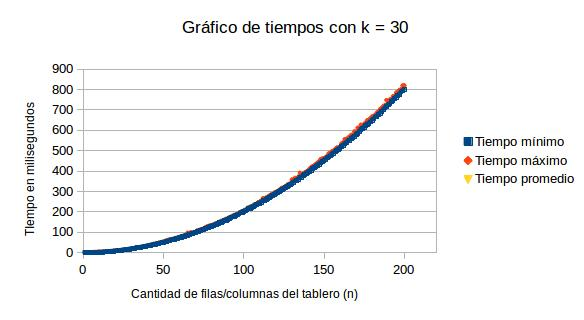
\includegraphics[width=\textwidth]{conjAcurva.jpg}\caption{Podemos ver como la curva roja que representa el tiempo máximo, sobresale por encima de la azul, que representa el mínimo, en varias partes del gráfico. La curva que representa el tiempo promedio esta entre las otras dos, por lo cual no se puede ver. Notemos que el gráfico es una curva, que podría o no ser $kn^2$ por alguna constante.}
\end{figure}
\pagebreak
\begin{figure}[h!]
\centering
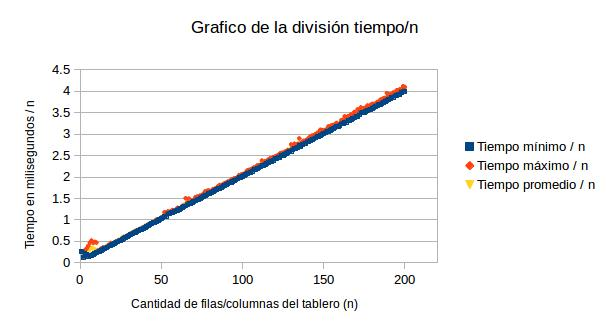
\includegraphics[width=\textwidth]{conjAlinea.jpg}\caption{Este gráfico lo hicimos para corroborar que, el gráfico anterior era efectivamente una curva del tipo $kn^2$ por una constante. Lo que hicimos fue dividir los tiempos obtenidos por la cantidad de filas/columnas (el n) de cada instancias, para ver si nos quedaba algo de la forma $nk$. Como estamos en el conjunto en el cual $k$ es una constante, lo que nos queda es $n$ por una constante que es una recta.}
\end{figure}
\begin{figure}[h!]
\centering
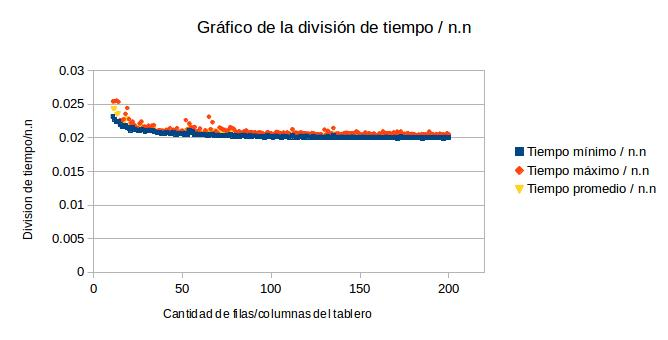
\includegraphics[width=\textwidth]{conjAconst.jpg}\caption{Finalmente, para asegurarnos de que las mediciones estén reflejando la complejidad, efectuamos otra división. Esta vez dividimos los tiempos por $n^2$, y vemos como el gráfico tiende a una constante $\simeq 0.020$, verificando así que el gráfico anterior es lineal. Como nuestro objetivo es ver como son los tiempos a medida que el $n$ aumenta, hemos descartado los primeros 11 valores ya que eran muy distintos a los demás y lo que queremos evaluar es el comportamiento asintótico.}
\end{figure}

\begin{figure}[h!]
\centering
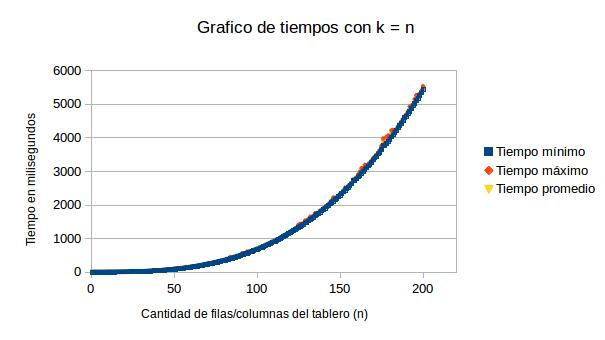
\includegraphics[width=\textwidth]{conjBcurva.jpg}\caption{Vemos que el gráfico es una curva también, pero esta vez alcanza valores mucho más grandes. Esto es muy razonable ya que antes, para $n = 170$ por ejemplo, teníamos 30 caballos, ahora para $n = 170$ vamos a tener 170 caballos. Si esta curva refleja la complejidad teórica, debería ser el gráfico de $kn^2$ y, como $k$ varia igual que $n$, quedaría $n^3$ por alguna constante. Veamos que tanto nos podemos asegurar de que esto es así con los siguientes gráficos.}
\centering
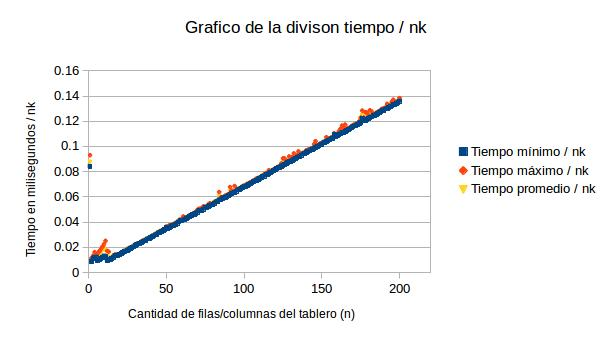
\includegraphics[width=\textwidth]{conjBlinea.jpg}\caption{Al igual que hicimos anteriormente, dividimos los tiempos obtenidos. La diferencia es que ahora por $nk$, ya que si solo dividimos por $n$ nos quedaría $kn$ y como $k$ varía igual que $n$ nos quedaría una curva y no es lo que queremos. Nuevamente podemos ver como el tiempo máximo supera al mínimo y el gráfico se asemeja mucho a una recta.}
\end{figure}
\pagebreak
\newpage
\begin{figure}[h!]
\centering
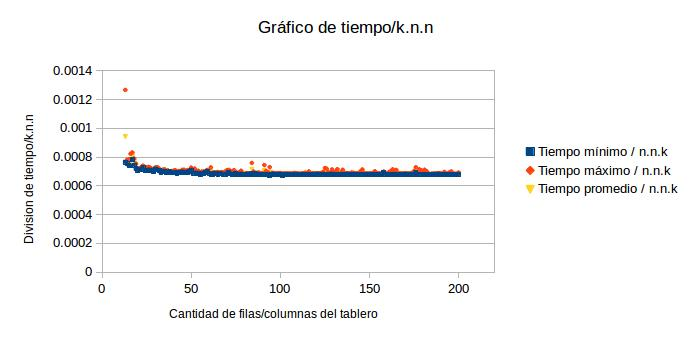
\includegraphics[width=\textwidth]{conjBconst13.jpg}\caption{Para asegurarnos aún más que el gráfico anterior era una recta, hicimos lo mismo que antes: dividimos el tiempo obtenido una vez más pero ahora por $k.n.n$. Al igual que antes, decidimos en este caso, no tomar algunos valores del principio y gráficar a partir de $n = 13$. Podemos apreciar que el gráfico tiende a una constante $\simeq 0.00068$.}
\end{figure}



\end{document}